
\documentclass[twoside]{book}
\usepackage[]{graphicx}\usepackage[]{xcolor}
%% maxwidth is the original width if it is less than linewidth
%% otherwise use linewidth (to make sure the graphics do not exceed the margin)
\makeatletter
\def\maxwidth{ %
  \ifdim\Gin@nat@width>\linewidth
    \linewidth
  \else
    \Gin@nat@width
  \fi
}
\makeatother

\definecolor{fgcolor}{rgb}{0.345, 0.345, 0.345}
\newcommand{\hlnum}[1]{\textcolor[rgb]{0.686,0.059,0.569}{#1}}%
\newcommand{\hlstr}[1]{\textcolor[rgb]{0.192,0.494,0.8}{#1}}%
\newcommand{\hlcom}[1]{\textcolor[rgb]{0.678,0.584,0.686}{\textit{#1}}}%
\newcommand{\hlopt}[1]{\textcolor[rgb]{0,0,0}{#1}}%
\newcommand{\hlstd}[1]{\textcolor[rgb]{0.345,0.345,0.345}{#1}}%
\newcommand{\hlkwa}[1]{\textcolor[rgb]{0.161,0.373,0.58}{\textbf{#1}}}%
\newcommand{\hlkwb}[1]{\textcolor[rgb]{0.69,0.353,0.396}{#1}}%
\newcommand{\hlkwc}[1]{\textcolor[rgb]{0.333,0.667,0.333}{#1}}%
\newcommand{\hlkwd}[1]{\textcolor[rgb]{0.737,0.353,0.396}{\textbf{#1}}}%

\usepackage{framed}
\makeatletter
\newenvironment{kframe}{%
 \def\at@end@of@kframe{}%
 \ifinner\ifhmode%
  \def\at@end@of@kframe{\end{minipage}}%
  \begin{minipage}{\columnwidth}%
 \fi\fi%
 \def\FrameCommand##1{\hskip\@totalleftmargin \hskip-\fboxsep
 \colorbox{shadecolor}{##1}\hskip-\fboxsep
     % There is no \\@totalrightmargin, so:
     \hskip-\linewidth \hskip-\@totalleftmargin \hskip\columnwidth}%
 \MakeFramed {\advance\hsize-\width
   \@totalleftmargin\z@ \linewidth\hsize
   \@setminipage}}%
 {\par\unskip\endMakeFramed%
 \at@end@of@kframe}
\makeatother

\definecolor{shadecolor}{rgb}{.97, .97, .97}
\definecolor{messagecolor}{rgb}{0, 0, 0}
\definecolor{warningcolor}{rgb}{1, 0, 1}
\definecolor{errorcolor}{rgb}{1, 0, 0}
\newenvironment{knitrout}{}{} % an empty environment to be redefined in TeX

\usepackage{alltt}
\newcommand{\SweaveOpts}[1]{}  % do not interfere with LaTeX
\newcommand{\SweaveInput}[1]{} % because they are not real TeX commands
\newcommand{\Sexpr}[1]{}       % will only be parsed by R


\usepackage[margin=.9in]{geometry}
%\usepackage{kpfonts}   % for \varhearsuit
%\usepackage{txfonts}    % for \varhearsuit
\usepackage{amsmath}
\usepackage{probstat}
\usepackage{booktabs}
\def\Tri{\distribution{Triangle}}
\def\Rayleigh{\distribution{Rayleigh}}
\def\SD{\operatorname{SD}}
\usepackage{xstring}
\usepackage{makeidx}

%\def\Prob{\operatorname{Pr}}
\def\tnot{\operatorname{not}}
\usepackage{hyperref}
\usepackage{graphicx}
\usepackage{tikz}
\usetikzlibrary{patterns}
\usepackage[hidenotes]{authNote}
\usepackage[answerdelayed,exercisedelayed,lastexercise,chapter]{problems}

%\def\myindex#1{\relax}
%\def\Rindex#1{\relax}
\def\myindex#1{\index{#1}}

\usepackage{multicol}
\usepackage{longtable}
\renewcommand{\arraystretch}{1.4}

\def\sfrac#1#2{#1/#2}
\newcommand{\Partial}[2]{\frac{\partial #1}{\partial #2}}


\usepackage[Bjornstrup]{fncychap}
\usepackage{fancyhdr}
\pagestyle{fancy}
\fancyhf{}

%% Now begin customising things. See the fancyhdr docs for more info.

\renewcommand{\chaptermark}[1]{\thispagestyle{fancy}\markboth{{#1}}{}}
\renewcommand{\sectionmark}[1]{\markright{{#1}}{}}
%\renewcommand{\headrulewidth}{0pt}

\newcommand{\exampleidx}[1]{{\it #1}}
\newcommand{\defidx}[1]{{\bf #1}}
\newcommand{\mainidx}[1]{{\bf #1}}
\newcommand{\probidx}[1]{{{\underline{#1}}}}

\newcommand{\variable}[1]{{\color{green!50!black}\texttt{#1}}}
%\newcommand{\dataframe}[1]{{\color{blue!80!black}\texttt{#1}}}
%\newcommand{\Rindex}[2][black]{\index{{\color{#1}\texttt{#2}}}}
\newcommand{\Rindex}[1]{\index{\texttt{#1}}}
\newcommand{\dataframe}[1]{{\color{blue!80!black}\texttt{#1}}\Rindex{#1}}
\newcommand{\function}[1]{{\color{purple!75!blue}\texttt{\StrSubstitute{#1}{()}{}()}}\Rindex{#1}}
\newcommand{\option}[1]{{\color{brown!80!black}\texttt{#1}}}
\newcommand{\argument}[1]{{\color{brown!80!black}\texttt{#1}}}
%\newcommand{\pkg}[1]{{\color{red!80!black}\texttt{#1}}}
\newcommand{\pkg}[1]{{\color{red!80!black}\texttt{#1}}\Rindex{#1}}
\renewcommand{\code}[1]{{\color{blue!80!black}\texttt{#1}}}
% and for models
\newcommand{\model}[2]{{$\,$\hbox{#1}\ \ensuremath{\sim}\ \hbox{#2}}}

\DeclareSymbolFont{extraup}{U}{zavm}{m}{n}
\DeclareMathSymbol{\varheartsuit}{\mathalpha}{extraup}{86}
\DeclareMathSymbol{\vardiamondsuit}{\mathalpha}{extraup}{87}

\chead{}
\lhead[\sf \thepage]{\sf \leftmark}
\rhead[\sf \leftmark]{\sf \thepage}
\lhead[\sf \thepage]{\sf \thechapter. \leftmark}
\rhead[\sf \thechapter. \leftmark]{\sf \thepage}
\cfoot{}
\lfoot[\sf Last Modified: \today]{\sf Math 241 : Spring 2014 : Pruim}
\rfoot[\sf Math 241 : Spring 2014 : Pruim]{\sf Last Modified: \today}

\pagestyle{fancy}

\usepackage{sfsect}
\usepackage{relsize}

%%%%%%%%%%%%%%%%%%%%%%%%%%%%%%% macros %%%%%%%%%%%%%%%%%%%%%%%%%%%%%%%%%%%%%%%%%%

\def\Chapter#1{%
\chapter{#1}
%\setcounter{page}{1}%
}
\def\R{{\sf R}}
\def\Rstudio{{\sf RStudio}}
\def\term#1{\textbf{#1}}
\def\tab#1{{\sf #1}}


\newlength{\tempfmlength}
\newsavebox{\fmbox}
\newenvironment{fmpage}[1]
     {
	 \medskip
	 \setlength{\tempfmlength}{#1}
	 \begin{lrbox}{\fmbox}
	   \begin{minipage}{#1}
		 \vspace*{.02\tempfmlength}
		 \hfill
	   \begin{minipage}{.95 \tempfmlength}}
		 {\end{minipage}\hfill
		 \vspace*{.015\tempfmlength}
		 \end{minipage}\end{lrbox}\fbox{\usebox{\fmbox}}
	 \medskip
	 }


\newenvironment{boxedText}[1][.98\textwidth]%
{%
\begin{center}
\begin{fmpage}{#1}
}%
{%
\end{fmpage}
\end{center}
}

\newenvironment{boxedTable}[2][tbp]%
{%
\begin{table}[#1]
  \refstepcounter{table}
  \begin{center}
\begin{fmpage}{.98\textwidth}
  \begin{center}
	\sf \large Box~\expandafter\thetable. #2
\end{center}
\medskip
}%
{%
\end{fmpage}
\end{center}
\end{table}		% need to do something about exercises that follow boxedTable
}

\def\question{{\sf Q. }}
\def\answer{{\sf A. }}

\newcounter{example}[section]

\newenvironment{example}%
{\refstepcounter{example}%
\textbf{Example \thesection.\arabic{example}. }}%
{}

\newenvironment{examples}%
{\refstepcounter{example}%
\textbf{Examples \thesection.\arabic{example}. }}%
{}

\renewcommand{\theexample}{\thesection.\arabic{example}}



\newif\ifsolutions
\solutionstrue
\solutionsfalse

\newif\ifsolutionslocal
\solutionslocaltrue
\solutionslocalfalse

\parindent=0pt
\parskip=3mm



\begin{knitrout}
\definecolor{shadecolor}{rgb}{0.969, 0.969, 0.969}\color{fgcolor}\begin{kframe}


{\ttfamily\noindent\color{warningcolor}{\#\# Warning in library(package, lib.loc = lib.loc, character.only = TRUE, logical.return = TRUE, : there is no package called 'DAAG'}}

{\ttfamily\noindent\color{warningcolor}{\#\# Warning in library(package, lib.loc = lib.loc, character.only = TRUE, logical.return = TRUE, : there is no package called 'abd'}}

{\ttfamily\noindent\color{warningcolor}{\#\# Warning in library(package, lib.loc = lib.loc, character.only = TRUE, logical.return = TRUE, : there is no package called 'alr3'}}\end{kframe}
\end{knitrout}

%%%%%%%%%%%%%%%%%%%%%% title page info %%%%%%%%%%%%%%%%%%%%%%%%%%%%%%

\title{Math 241: Statistics for the Physical Sciences and Engineering}

\author{R Pruim}

\date{Spring 2014}

%%%%%%%%%%%%%%%%%%%%%%%%%%%%%%%%%%%%%%%%%%%%%%%%%%%%%%%%%%%%%%%%%%%%%
\makeindex
%%%%%%%%%%%%%%%%%%%%%%%%%%%%%%%%%%%%%%%%%%%%%%%%%%%%%%%%%%%%%%%%%%%%%

\lhead[\sf \thepage]{\sf \thechapter. \leftmark}
\rhead[\sf \thechapter. \leftmark]{\sf \thepage}



\begin{document}


\chapter{Hypothesis Testing}

\section{The Lady Tasting Tea}

\myindex{lady tasting tea|exampleidx}%
%\myindex{tea|seeonly{lady tasting tea}}%
There is a famous story about a lady who claimed that
tea with milk tasted different depending on whether the milk was 
added to the tea or the tea added to the milk.
The story is famous because of the setting in which she made this claim.  
She was attending a party in Cambridge, England, in the $1920$s.
Also in attendance were a number of university dons and their wives.
The scientists in attendance scoffed at the woman and her claim.
What, after all, could be the difference?

\myindex{Fisher, R. A.}%
All the scientists but one, that is.  Rather than simply dismiss the 
woman's claim, he proposed that they decide how one 
should \emph{test} the claim.  The tenor of the conversation changed at 
this suggestion, and the scientists began to discuss how the claim should be 
tested.  Within a few minutes cups of tea with milk had been prepared and 
presented to the woman for tasting.

Let's take this simple example as a prototype for a statistical study.
What steps are involved?  
\begin{enumerate}
  \item Determine the question of interest.

	Just what is it we want to know?  It may take some effort to 
	make a vague idea precise.  The precise questions may not exactly
	correspond to our vague questions, and the very exercise of 
	stating the question precisely may modify our question.  Sometimes
	we cannot come up with any way to answer the question we really want
	to answer, so we have to live with some other question that is 
	not exactly what we wanted but is something we can study and will
	(we hope) give us some information about our original question.

	In our example this question seems fairly easy to state:
	Can the lady tell the difference between the two tea preparations?
	But we need to refine this question.  For example, are we 
	asking if she \emph{always} correctly identifies cups of tea
	or merely if she does better than we could do ourselves (by 
	guessing)?  

  \item 
	Determine the \term{population}. 
	\myindex{population}%

	Just who or what do we want to know about?  Are we only interested in
	this one woman or women in general or only women who claim to
	be able to distinguish tea preparations?

  \item
	Select \term{measurements}.

	We are going to need some data.  
	We get our data by making some measurements.
	These might be physical measurements with some device (like a ruler
	or a scale).
	But there are other sorts of measurements too, 
	like the answer to a question on a form.
	Sometimes it is tricky to figure out just what to measure.
	(How do we measure happiness or intelligence, for example?)
	Just how we do our measuring will have important consequences 
	for the subsequent statistical analysis.
	The recorded values of these measurements are called
	\term{variables} (because the values vary from one individual to another).

	In our example, a measurement may consist of recording for a given
	cup of tea whether the woman's claim is correct or incorrect.
	%it is milk-into-tea or tea-into-milk.

  \item
	Determine the \term{sample}.
	\myindex{sample}%

	Usually we cannot measure every individual in our population; we have 
	to select some to measure.  
	But how many and which ones?  
	These are important questions that must be answered.
	Generally speaking, bigger is better, but it is also more expensive.
	Moreover, no size is large enough if the sample is selected inappropriately.

	Suppose we gave the lady one cup of tea.  If she correctly identifies
	the mixing procedure, will we be convinced of her claim?  She might just
	be guessing; so we should probably have her taste more than one 
	cup.  Will we be convinced if she correctly identifies $5$ cups? $10$ cups?
	$50$ cups?

	What if she makes a mistake?  If we present her with $10$ cups and she
	correctly identifies $9$ of the $10$, what will we conclude?  
	\authNote{added A success rate of -- 2010-10-23}%
	A success rate of $90$\% is, it seems,
	much better than just guessing, and anyone can make a mistake now and then.
	But what if she correctly identifies $8$ out of $10$? $80$ out of $100$?
	
	And how should we prepare the cups?  Should we make $5$ each way?  
	\authNote{Left it as "and how" -- 2010-10-23}%
	Does it matter if we tell the woman that there are $5$ prepared 
	each way?
	Should we flip a coin to decide even if that means we might end 
	up with $3$ prepared one way and $7$ the other way?  
	Do any of these differences matter?

  \item
	Make and record the measurements.

	Once we have the design figured out, we have to do the legwork of 
	data collection.  This can be a time-consuming and tedious process.
	In the case of the lady tasting tea, the scientists decided to 
	present her with ten cups of tea which were quickly prepared.
	A study of public opinion may require many thousands of phone calls or 
	personal interviews.
	In a laboratory setting, each measurement might be the result 
	of a carefully performed laboratory experiment.

  \item Organize the data.

	Once the data have been collected, it is often necessary or useful
	to organize them.  Data are typically stored in spreadsheets or 
	in other formats that are convenient for processing with 
	statistical packages.  Very large data sets are often stored in 
	databases.  
	
	Part of the organization of the data may involve producing graphical and
	numerical summaries of the data.  These summaries may give us initial
	insights into our questions or help us detect errors that may have occurred
	to this point.

  \item Draw conclusions from data.

	Once the data have been collected, organized, and analyzed, we need
	to reach a conclusion.  
	Do we believe the woman's claim?  
	Or do we think she is merely guessing?  How sure are we that this
	conclusion is correct?

%	In Parts~\ref{part:inf1}--\ref{part:inf2} 
	Eventually we will
	learn a number of important and frequently used methods for 
	drawing inferences from data.  More importantly, we will learn
	the basic framework used for such procedures so that it should 
	become easier and easier to learn new procedures as we become 
	familiar with the framework.
	
	%How strongly do we believe it?  

  \item Produce a report.

		Typically the results of a statistical study are reported in 
		some manner.  This may be as a refereed article in an academic 
		journal, as an internal report to a company, or as a solution
		to a problem on a homework assignment.  These reports may themselves
		be further distilled into press releases, newspaper articles,
		advertisements, and the like.  The mark of a good report
		is that it provides the essential information about each 
		of the steps of the study.

		As we go along, we will learn some of the standard terminology and
		procedures that you are likely to see in basic statistical reports and 
		will gain a framework for learning more.  
\end{enumerate}

At this point, you may be wondering who the innovative scientist was and 
what the results of the experiment were.
\myindex{Fisher, R. A.}%
The scientist was R. A. Fisher, who first described this situation
as a pedagogical example in his 1925 book on 
statistical methodology \cite{Fisher:1925:Methods}.
Fisher developed statistical methods that are among the most
important and widely used methods to this day, and most of his 
applications were biological.
\nocite{Fisher:1970:Methods}%


\section{Coins and Cups}
You might also be curious about how the experiment came out.
How many cups of tea were prepared?  How many did the woman 
correctly identify?  What was the conclusion?

Fisher never says.  In his book he is interested in the method, not the 
particular results.  But let's suppose we decide to test the lady with
ten cups of tea.  
We'll flip a coin to decide which way to prepare the cups.  
If we flip a head, we will pour the milk in first; if tails, we 
put the tea in first.
Then we present the ten cups to the lady and have her state which ones she
thinks were prepared each way.  

It is easy to give her a score (9 out of 10, or 7 out of 10, or whatever
it happens to be).  It is trickier to figure out what to do with her score.
Even if she is just guessing and has no idea, she could get lucky and 
get quite a few correct -- maybe even all 10.  But how likely is that?

Let's try an experiment.  I'll flip 10 coins.  You guess which are heads and
which are tails, and we'll see how you do.  

$\vdots$

Comparing with your classmates, we will undoubtedly see that some 
of you did better and others worse.

Now let's suppose the lady gets 9 out of 10 correct.  That's not perfect,
but it is better than we would expect for someone who was just guessing.
On the other hand, it is not impossible to get 9 out of 10 just by guessing.
So here is Fisher's great idea:  Let's figure out how hard it is to get
9 out of 10 by guessing.  If it's not so hard to do, then perhaps that's 
just what happened, so we won't be too impressed with the lady's tea tasting
ability.  On the other hand, if it is really unusual to get 9 out of 10 
correct by guessing, then we will have some evidence that she must 
be able to tell something.

But how do we figure out how unusual it is to get 9 out of 10 just by 
guessing?  We'll learn another method later, but for now, let's just 
flip a bunch of coins and keep track.  If the lady is just guessing, she 
might as well be flipping a coin.

So here's the plan.  We'll flip 10 coins.  We'll call the heads correct 
guesses and the tails incorrect guesses.  Then we'll flip 10 more coins,
and 10 more, and 10 more, and \dots.  That would get pretty tedious.
Fortunately, computers are good at tedious things, so we'll let the computer 
do the flipping for us using a tool in the \pkg{mosaic} package.
%This package is already installed in our \RStudio\ server.  If you are running
%your own installation of \R\ you can install \pkg{mosaic} using the following 
%command:
%<<install-mosaic,eval=FALSE>>=
%install.packages("mosaic")
%@
The \function{rflip()} function can flip one coin

\begin{knitrout}
\definecolor{shadecolor}{rgb}{0.969, 0.969, 0.969}\color{fgcolor}\begin{kframe}
\begin{alltt}
\hlkwd{require}\hlstd{(mosaic)}
\hlkwd{rflip}\hlstd{()}
\end{alltt}
\begin{verbatim}
## 
## Flipping 1 coin [ Prob(Heads) = 0.5 ] ...
## 
## T
## 
## Number of Heads: 0 [Proportion Heads: 0]
\end{verbatim}
\end{kframe}
\end{knitrout}
or a number of coins
\begin{knitrout}
\definecolor{shadecolor}{rgb}{0.969, 0.969, 0.969}\color{fgcolor}\begin{kframe}
\begin{alltt}
\hlkwd{rflip}\hlstd{(}\hlnum{10}\hlstd{)}
\end{alltt}
\begin{verbatim}
## 
## Flipping 10 coins [ Prob(Heads) = 0.5 ] ...
## 
## H H H H H H T T T H
## 
## Number of Heads: 7 [Proportion Heads: 0.7]
\end{verbatim}
\end{kframe}
\end{knitrout}
and show us the results.

Typing \code{rflip(10)} a bunch of times is almost as tedious as 
flipping all those coins.   But it is not too hard to 
tell \R\ to \function{do()} this a bunch of times.
\begin{knitrout}
\definecolor{shadecolor}{rgb}{0.969, 0.969, 0.969}\color{fgcolor}\begin{kframe}
\begin{alltt}
\hlkwd{do}\hlstd{(}\hlnum{2}\hlstd{)} \hlopt{*} \hlkwd{rflip}\hlstd{(}\hlnum{10}\hlstd{)}
\end{alltt}
\begin{verbatim}
##    n heads tails prop
## 1 10     5     5  0.5
## 2 10     5     5  0.5
\end{verbatim}
\end{kframe}
\end{knitrout}
Let's get \R\ to \function{do()} it for us 10,000 times and make 
a table and a histogram of the results.

\begin{knitrout}
\definecolor{shadecolor}{rgb}{0.969, 0.969, 0.969}\color{fgcolor}\begin{kframe}
\begin{alltt}
\hlstd{results} \hlkwb{<-} \hlkwd{do}\hlstd{(}\hlnum{10000}\hlstd{)} \hlopt{*} \hlkwd{rflip}\hlstd{(}\hlnum{10}\hlstd{)}
\hlkwd{table}\hlstd{(results}\hlopt{$}\hlstd{heads)}
\end{alltt}
\begin{verbatim}
## 
##    0    1    2    3    4    5    6    7    8    9   10 
##    5  102  467 1203 2048 2470 2035 1140  415  108    7
\end{verbatim}
\begin{alltt}
\hlkwd{histogram}\hlstd{(}\hlopt{~}\hlstd{heads,} \hlkwc{data} \hlstd{= results,} \hlkwc{width} \hlstd{=} \hlnum{1}\hlstd{)}
\end{alltt}
\end{kframe}

{\centering 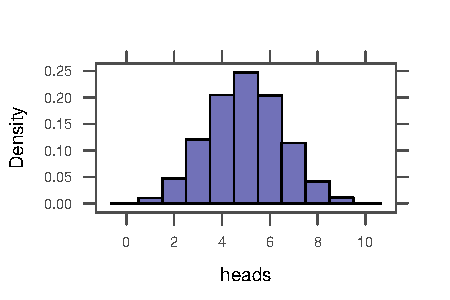
\includegraphics[width=\maxwidth]{figures/fig-flip4-1} 

}



\end{knitrout}
\begin{knitrout}
\definecolor{shadecolor}{rgb}{0.969, 0.969, 0.969}\color{fgcolor}\begin{kframe}
\begin{alltt}
\hlkwd{perctable}\hlstd{(results}\hlopt{$}\hlstd{heads)}  \hlcom{#  the table in percents}
\end{alltt}
\begin{verbatim}
## 
##     0     1     2     3     4     5     6     7     8     9    10 
##  0.05  1.02  4.67 12.03 20.48 24.70 20.35 11.40  4.15  1.08  0.07
\end{verbatim}
\begin{alltt}
\hlkwd{proptable}\hlstd{(results}\hlopt{$}\hlstd{heads)}  \hlcom{#  the table in proportions (i.e., decimals)}
\end{alltt}
\begin{verbatim}
## 
##      0      1      2      3      4      5      6      7      8      9     10 
## 0.0005 0.0102 0.0467 0.1203 0.2048 0.2470 0.2035 0.1140 0.0415 0.0108 0.0007
\end{verbatim}
\end{kframe}
\end{knitrout}
We could also use \function{tally()} for this.
\begin{knitrout}
\definecolor{shadecolor}{rgb}{0.969, 0.969, 0.969}\color{fgcolor}\begin{kframe}
\begin{alltt}
\hlkwd{tally}\hlstd{(}\hlopt{~}\hlstd{heads,} \hlkwc{data} \hlstd{= results)}
\end{alltt}
\begin{verbatim}
## 
##    0    1    2    3    4    5    6    7    8    9   10 
##    5  102  467 1203 2048 2470 2035 1140  415  108    7
\end{verbatim}
\begin{alltt}
\hlkwd{tally}\hlstd{(}\hlopt{~}\hlstd{heads,} \hlkwc{data} \hlstd{= results,} \hlkwc{format} \hlstd{=} \hlstr{"percent"}\hlstd{)}
\end{alltt}
\begin{verbatim}
## 
##     0     1     2     3     4     5     6     7     8     9    10 
##  0.05  1.02  4.67 12.03 20.48 24.70 20.35 11.40  4.15  1.08  0.07
\end{verbatim}
\begin{alltt}
\hlkwd{tally}\hlstd{(}\hlopt{~}\hlstd{heads,} \hlkwc{data} \hlstd{= results,} \hlkwc{format} \hlstd{=} \hlstr{"proportion"}\hlstd{)}
\end{alltt}
\begin{verbatim}
## 
##      0      1      2      3      4      5      6      7      8      9     10 
## 0.0005 0.0102 0.0467 0.1203 0.2048 0.2470 0.2035 0.1140 0.0415 0.0108 0.0007
\end{verbatim}
\end{kframe}
\end{knitrout}


You might be surprised to see that the number of correct guesses
is exactly 5 (half of the 10 tries) only 
25\%
of the time.  But most of the results are quite close to 5 correct.
67\% of the results are 
4, 5, or 6, for example.
And 1\% of the results 
are  between 3 and 7 (inclusive).
But getting 8 correct is a bit unusual, and getting 9 or 10 correct is even 
more unusual.  

So what do we conclude?  It is possible that the lady could get 9 or 10 correct
just by guessing, but it is not very likely (it only happened in about
1.2\% of our simulations). 
So \emph{one of two things must be true}:
\begin{itemize}
\item The lady got unusually ``lucky", or 
\item The lady is not just guessing.
\end{itemize}

Although Fisher did not say how the experiment came out, others have reported
that the lady correctly identified all 10 cups!
\cite{salsburg}

This same reasoning can be applied to answer a wide range of questions that
have a similar form.  For example, the question of whether dogs can smell
cancer could be answered essentially the same way (although it would be a bit
more involved than preparing tea and presenting cups to the Lady).




\section{A General Framework}


\begin{description}
	\item[hypothesis] A statement that can be true or false.
	\item[statistical hypothesis] A hypothesis about a parameter or parameters.
\end{description}

\begin{examples}
	The following are examples of null hypotheses.
	\begin{enumerate}
		\item
			$\mu = 0$.  (The population mean is 0.)
		\item
			$\beta_1=0$.  (The ``true'' slope is 0 -- assuming a model like $\E(Y) = \beta_0 + \beta_1 x$.)
		\item
			$\beta_1 = \beta_2$ (Two parameters in the model are equal.)
		\item
			$\beta_2 = \beta_3 = 0$ (Two parameters in the model are both equal to 0.)
	\end{enumerate}
\end{examples}

\subsection{The Four Step Process}
Hypothesis testing generally follows a four-step process.
\begin{enumerate}
	\item 
		State the null and alternative hypotheses.

		The null hypothesis is on trial and innocent until proven guilty.  We will
		render one of two verdicts:  Reject the null hypothesis (guilty) or do not reject
		the null hypothesis (not guilty).  

	\item
		Compute a test statistic.

		All the evidence against the null hypothesis must be summarized in a
		single number called the test statistic.  It is a statistic because 
		it is a number computed from the data.  It is called a test statistic
		because we are using it to do hypothesis testing.

	\item
		Determine the p-value.

		The p-value is a probability:  Assuming the null hypothesis is true,
		how likely are we to get at least as much evidence against it (i.e., a
		test statistic as anusual as the one observed) just by random chance?

	\item
		Interpret the results.

		If the p-value is small, then one of two things is true:
		\begin{enumerate}
			\item The null hypothesis is true and something unlikely occurred
				in our sample, or 
			\item The null hypothesis is false (and the
				p-value is a counter-factual probability).
		\end{enumerate}
		For this reason we consider small p-values as evidence against the null
		hypothesis.
\end{enumerate}

\subsection{The Lady Tasting Tea, Revisted}
\begin{example}
\label{example:lady-binom}
For the lady tasting tea, this process looks like
\begin{enumerate}
	\item
		$H_0$: The probability of being correct is $0.5$ (she's just guessing).

		$H_a$ The probability of being correct is larger than $0.5$ (she can do
		better than someone who just guesses).
	\item
		Test statistic: $x=9$ of $n=10$ were correct.
	\item
		P-value

		\begin{enumerate}
			\item
				Based on our empirical method, we estimate a p-value of
\begin{knitrout}
\definecolor{shadecolor}{rgb}{0.969, 0.969, 0.969}\color{fgcolor}\begin{kframe}
\begin{alltt}
\hlkwd{prop}\hlstd{(}\hlopt{~}\hlstd{(heads} \hlopt{>=} \hlnum{9}\hlstd{),} \hlkwc{data} \hlstd{= results)}
\end{alltt}


{\ttfamily\noindent\itshape\color{messagecolor}{\#\#\ \ \ \  target level: TRUE;\ \ other levels: FALSE}}\begin{verbatim}
##   TRUE 
## 0.0115
\end{verbatim}
\end{kframe}
\end{knitrout}

	\item
		The probabilities for the number of correct guesses 
		can be worked out theoretically as well.  The resulting distribution
		is called a \term{binomial} distribution.  As with other distributions we 
		have seen, \R\ includes the functions 
		\function{dbinom()}, 
		\function{pbinom()}, 
		\function{qbinom()}, and 
		\function{rbinom()}. 
\begin{knitrout}
\definecolor{shadecolor}{rgb}{0.969, 0.969, 0.969}\color{fgcolor}\begin{kframe}
\begin{alltt}
\hlkwd{plotDist}\hlstd{(}\hlstr{"binom"}\hlstd{,} \hlkwc{size} \hlstd{=} \hlnum{10}\hlstd{,} \hlkwc{prob} \hlstd{=} \hlnum{0.5}\hlstd{)}  \hlcom{# size = # of flips; prob=probability of heads}
\hlkwd{dbinom}\hlstd{(}\hlnum{9}\hlstd{,} \hlnum{10}\hlstd{,} \hlnum{0.5}\hlstd{)} \hlopt{+} \hlkwd{dbinom}\hlstd{(}\hlnum{10}\hlstd{,} \hlnum{10}\hlstd{,} \hlnum{0.5}\hlstd{)}
\end{alltt}
\begin{verbatim}
## [1] 0.01074219
\end{verbatim}
\begin{alltt}
\hlnum{1} \hlopt{-} \hlkwd{pbinom}\hlstd{(}\hlnum{8}\hlstd{,} \hlnum{10}\hlstd{,} \hlnum{0.5}\hlstd{)}  \hlcom{# Note: P(X >=9) = 1 - P(X <=8)}
\end{alltt}
\begin{verbatim}
## [1] 0.01074219
\end{verbatim}
\end{kframe}

{\centering 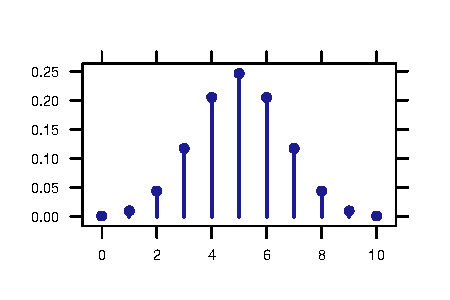
\includegraphics[width=\maxwidth]{figures/fig-unnamed-chunk-2-1} 

}



\end{knitrout}
\end{enumerate}
\item Interpret the p-value.

	The p-value is fairly small.  While it is possible that the woman is just guessing,
	it would be pretty unlikely for a guesser to do this well, so we reject the 
	null hypothesis.

\end{enumerate}
\end{example}

\begin{example}
	This situation is so common that there is a function to do the calculations for us.
	We just need to provide the values of $x$ and $n$:
\begin{knitrout}
\definecolor{shadecolor}{rgb}{0.969, 0.969, 0.969}\color{fgcolor}\begin{kframe}
\begin{alltt}
\hlkwd{binom.test}\hlstd{(}\hlkwc{x} \hlstd{=} \hlnum{9}\hlstd{,} \hlkwc{n} \hlstd{=} \hlnum{10}\hlstd{)}  \hlcom{# default test is 2-sided}
\end{alltt}
\begin{verbatim}
## 
## 	Exact binomial test
## 
## data:  x and n
## number of successes = 9, number of trials = 10, p-value = 0.02148
## alternative hypothesis: true probability of success is not equal to 0.5
## 95 percent confidence interval:
##  0.5549839 0.9974714
## sample estimates:
## probability of success 
##                    0.9
\end{verbatim}
\end{kframe}
\end{knitrout}
	The output above doesn't match what we obtained in Example~\ref{example:lady-binom}
	because the alternative hypothesis is different.  It accepts both low number of correct
	identifications (0 or 1) and high numbers (9 or 10) as evidence against the null
	hypothesis.  If we want a one-sided p-value, we just need to ask:
\begin{knitrout}
\definecolor{shadecolor}{rgb}{0.969, 0.969, 0.969}\color{fgcolor}\begin{kframe}
\begin{alltt}
\hlkwd{binom.test}\hlstd{(}\hlkwc{x} \hlstd{=} \hlnum{9}\hlstd{,} \hlkwc{n} \hlstd{=} \hlnum{10}\hlstd{,} \hlkwc{alternative} \hlstd{=} \hlstr{"greater"}\hlstd{)}
\end{alltt}
\begin{verbatim}
## 
## 	Exact binomial test
## 
## data:  x and n
## number of successes = 9, number of trials = 10, p-value = 0.01074
## alternative hypothesis: true probability of success is greater than 0.5
## 95 percent confidence interval:
##  0.6058367 1.0000000
## sample estimates:
## probability of success 
##                    0.9
\end{verbatim}
\end{kframe}
\end{knitrout}

\end{example}


\section{T-tests}

Many hypothesis tests are based on a $t$-distribution.  These tests all use a similar sort
of test statistic:

\[
t = \frac{\mbox{estimate} - \mbox{hypothesized value}}{\mbox{standard error}}
\]

The numerator tells us that the more the estimate and the hypothesized value differ, 
the stronger the evidence.  The denominator tells us that differences mean more when the standard
deviation is small than when the standard deviation is large.

The test statistic is converted to a p-value by comparing it to the t-distribution with appropriate
degrees of freedom.  For linear models, this is the degrees of freedom associated with the 
residual standard error.

\subsection{The 1-sample t-test}
The 1-sample t-test tests the null hypothesis
\begin{itemize}
	\item $H_0: \mu = \mu_0$, vs.
	\item $H_a: \mu \neq 0$.
\end{itemize}
That is, it tests whether there is evidence that the mean of some population ($\mu$) is different
from some hypothesized value ($\mu_0$).

\begin{example}
Let's look at some data on weight loss programs.  In this data set, there were two groups.  One group
received a monetary incentive if they lost weight.  The controls
did not receive a monetary incentive.  Let's see whether on average the controls lost weight
\begin{knitrout}
\definecolor{shadecolor}{rgb}{0.969, 0.969, 0.969}\color{fgcolor}\begin{kframe}
\begin{alltt}
\hlkwd{require}\hlstd{(Stat2Data)}
\end{alltt}


{\ttfamily\noindent\itshape\color{messagecolor}{\#\# Loading required package: Stat2Data}}\begin{alltt}
\hlkwd{data}\hlstd{(WeightLossIncentive)}
\hlstd{Controls} \hlkwb{<-} \hlkwd{subset}\hlstd{(WeightLossIncentive, Group} \hlopt{==} \hlstr{"Control"}\hlstd{)}
\hlkwd{favstats}\hlstd{(}\hlopt{~}\hlstd{WeightLoss,} \hlkwc{data} \hlstd{= Controls)}
\end{alltt}
\begin{verbatim}
##  min Q1 median    Q3 max     mean       sd  n missing
##  -17 -2      3 11.25  20 3.921053 9.107785 19       0
\end{verbatim}
\end{kframe}
\end{knitrout}
The standard error when doing inference for a mean is 
\[
SE = \frac{s}{\sqrt{n}} = 
\frac{ 
	9.1077854
}{
	\sqrt{ 19 } 
}
=
2.0894693 
\]
\begin{knitrout}
\definecolor{shadecolor}{rgb}{0.969, 0.969, 0.969}\color{fgcolor}\begin{kframe}
\begin{alltt}
\hlstd{SE} \hlkwb{<-} \hlnum{9.108} \hlopt{/} \hlkwd{sqrt}\hlstd{(}\hlnum{19}\hlstd{); SE}
\end{alltt}
\begin{verbatim}
## [1] 2.089519
\end{verbatim}
\end{kframe}
\end{knitrout}
If we want to test our null hypothesis, then we compute a t-statistic:
\begin{knitrout}
\definecolor{shadecolor}{rgb}{0.969, 0.969, 0.969}\color{fgcolor}\begin{kframe}
\begin{alltt}
\hlstd{t} \hlkwb{<-} \hlstd{(}\hlnum{3.92} \hlopt{-} \hlnum{0}\hlstd{)} \hlopt{/} \hlstd{SE; t}
\end{alltt}
\begin{verbatim}
## [1] 1.87603
\end{verbatim}
\end{kframe}
\end{knitrout}
and from this a p-value, which is the tails probability for a t-distribution with 18 degrees of freedom.
\begin{knitrout}
\definecolor{shadecolor}{rgb}{0.969, 0.969, 0.969}\color{fgcolor}\begin{kframe}
\begin{alltt}
\hlnum{1} \hlopt{-} \hlkwd{pt}\hlstd{(t,} \hlkwc{df} \hlstd{=} \hlnum{19} \hlopt{-} \hlnum{1}\hlstd{)}
\end{alltt}
\begin{verbatim}
## [1] 0.03848197
\end{verbatim}
\begin{alltt}
\hlnum{2} \hlopt{*} \hlstd{(}\hlnum{1} \hlopt{-} \hlkwd{pt}\hlstd{(t,} \hlkwc{df} \hlstd{=} \hlnum{19} \hlopt{-} \hlnum{1}\hlstd{))}
\end{alltt}
\begin{verbatim}
## [1] 0.07696394
\end{verbatim}
\end{kframe}
\end{knitrout}
This p-value can also be generated from a linear model.
\begin{knitrout}
\definecolor{shadecolor}{rgb}{0.969, 0.969, 0.969}\color{fgcolor}\begin{kframe}
\begin{alltt}
\hlstd{model} \hlkwb{<-} \hlkwd{lm}\hlstd{(WeightLoss} \hlopt{~} \hlnum{1}\hlstd{,} \hlkwc{data} \hlstd{= Controls)}  \hlcom{# only an intercept term in the model}
\hlkwd{coef}\hlstd{(}\hlkwd{summary}\hlstd{(model))}
\end{alltt}
\begin{verbatim}
##             Estimate Std. Error  t value   Pr(>|t|)
## (Intercept) 3.921053   2.089469 1.876578 0.07688493
\end{verbatim}
\end{kframe}
\end{knitrout}
What is this model?
	\[
	Y = \beta_0 \cdot 1 + \varepsilon
	\]
So $\beta_0$ is the mean value of the response (\variable{WeightLoss}).

Either way, our p-value is $0.077$ (1 or 2 significant digits are sufficient for reporting 
p-values).  This is not
compelling evidence that the weight loss program actually leads to a change in weight.  A change this
large could occur just by chance in nearly 8\% of samples.
\end{example}

\begin{example}
Again, there is a function to automate this test:
\begin{knitrout}
\definecolor{shadecolor}{rgb}{0.969, 0.969, 0.969}\color{fgcolor}\begin{kframe}
\begin{alltt}
\hlkwd{t.test}\hlstd{(}\hlopt{~}\hlstd{WeightLoss,} \hlkwc{data} \hlstd{= Controls)}
\end{alltt}
\begin{verbatim}
## 
## 	One Sample t-test
## 
## data:  data$WeightLoss
## t = 1.8766, df = 18, p-value = 0.07688
## alternative hypothesis: true mean is not equal to 0
## 95 percent confidence interval:
##  -0.4687594  8.3108647
## sample estimates:
## mean of x 
##  3.921053
\end{verbatim}
\end{kframe}
\end{knitrout}
	If we don't want so much out put, we can cull out only the p-value:
\begin{knitrout}
\definecolor{shadecolor}{rgb}{0.969, 0.969, 0.969}\color{fgcolor}\begin{kframe}
\begin{alltt}
\hlkwd{pval}\hlstd{(}\hlkwd{t.test}\hlstd{(}\hlopt{~}\hlstd{WeightLoss,} \hlkwc{data} \hlstd{= Controls))}
\end{alltt}
\begin{verbatim}
##    p.value 
## 0.07688493
\end{verbatim}
\end{kframe}
\end{knitrout}
\end{example}

\subsection{Testing Model Coefficients}

\begin{example}
	Now let's compare the controls to the incentive group.  That is the question 
	the study was primarily interested in.
\begin{knitrout}
\definecolor{shadecolor}{rgb}{0.969, 0.969, 0.969}\color{fgcolor}\begin{kframe}
\begin{alltt}
\hlstd{model2} \hlkwb{<-} \hlkwd{lm}\hlstd{(WeightLoss} \hlopt{~} \hlstd{Group,} \hlkwc{data} \hlstd{= WeightLossIncentive)}
\end{alltt}
\end{kframe}
\end{knitrout}
	What is this model?
	\[
	Y = \beta_0 + \beta_1 x + \varepsilon
	\]
where $x$ is 0 for the controls and 1 for the incentive group.  That is, $Y \sim \Norm(\beta_0, \sigma)$
for the control group and $Y \sim \Norm(\beta_0 + \beta_1, \sigma)$ for the incentive group.
A test of the null hypothesis $\beta_1 = 0$ tests whether the two groups had different amounts 
of weight loss (on average).   (Note that this model also assumes that the two groups have the same 
standard deviation.  There are ways to test this hypothesis without that assumption.)
\begin{knitrout}
\definecolor{shadecolor}{rgb}{0.969, 0.969, 0.969}\color{fgcolor}\begin{kframe}
\begin{alltt}
\hlkwd{favstats}\hlstd{(WeightLoss} \hlopt{~} \hlstd{Group,} \hlkwc{data} \hlstd{= WeightLossIncentive)}
\end{alltt}
\begin{verbatim}
##      .group   min   Q1 median    Q3 max      mean       sd  n missing
## 1   Control -17.0 -2.0      3 11.25  20  3.921053 9.107785 19       0
## 2 Incentive  -0.5  7.5     18 24.00  30 15.676471 9.413988 17       2
\end{verbatim}
\begin{alltt}
\hlkwd{coef}\hlstd{(}\hlkwd{summary}\hlstd{(model2))}
\end{alltt}
\begin{verbatim}
##                 Estimate Std. Error  t value     Pr(>|t|)
## (Intercept)     3.921053   2.122817 1.847099 0.0734505837
## GroupIncentive 11.755418   3.089152 3.805387 0.0005635376
\end{verbatim}
\end{kframe}
\end{knitrout}
The small p-value provides evidence against the null hypothesis.  That is, we have evidence that
there is a difference between the mean amount of weight lost in the two groups.  (Those with a monetary
incentive lost more.)  
\end{example}

A difference large enough cause us to reject a null hypothesis of ``no difference" 
is called a \term{statistically significant} difference.  Differences may fail to be statistically
significant if they are small, if they are masked by underlying variability, or if there is too 
little data.  Good studies will collect enough data and work to reduce variability (if that is possible)
in order to have a reasonable expectation of detecting differences if they are large enough to 
be scientifically interesting.

\begin{example}
Suppose you suspect that drag force should be proportional to the square of velocity.  Let's see
if that is consistent with the data collected by some physics students.  
In this experiment, the students rigged up neutrally buoyant balloon and then loaded it 
with different amounts of weight and dropped it until and recorded its terminal velocity.
At that point the force due to gravity (determined by the mass loaded to the balloon) 
is equal to the drag force (because there is no acceleration).

We'll fit a power law model
\[
\variable{force.drag} = A \cdot \variable{velocity}^p
\]
and test the hypothesis that $p=2$.  We can fit this model using a log-log transformation:
\[
\log(\variable{force.drag}) = \log(A)  +  p \log( \variable{velocity} )
\]
So $p=\beta_1$ in our usual linear model notation.

\begin{knitrout}
\definecolor{shadecolor}{rgb}{0.969, 0.969, 0.969}\color{fgcolor}\begin{kframe}
\begin{alltt}
\hlstd{drag.model} \hlkwb{<-} \hlkwd{lm}\hlstd{(}\hlkwd{log}\hlstd{(force.drag)} \hlopt{~} \hlkwd{log}\hlstd{(velocity),} \hlkwc{data} \hlstd{= drag)}
\hlkwd{xyplot}\hlstd{(}\hlkwd{log}\hlstd{(force.drag)} \hlopt{~} \hlkwd{log}\hlstd{(velocity),} \hlkwc{data} \hlstd{= drag)}
\end{alltt}
\end{kframe}

{\centering 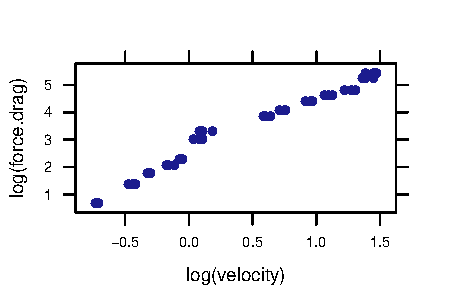
\includegraphics[width=\maxwidth]{figures/fig-drag-again-1} 

}



\end{knitrout}
The fit is not perfect, and in fact suggests a systematic problem with the way
these data were collected:%
\footnote{There is some evidence in this data that some of the observations did not reach
critical velocity.  
It would be good to refit this data with those observations removed from the data.
See Exercise~\ref{prob:drag-refit}.
}
\begin{knitrout}
\definecolor{shadecolor}{rgb}{0.969, 0.969, 0.969}\color{fgcolor}\begin{kframe}
\begin{alltt}
\hlkwd{xyplot}\hlstd{(}\hlkwd{resid}\hlstd{(drag.model)} \hlopt{~} \hlkwd{fitted}\hlstd{(drag.model))}
\hlkwd{qqmath}\hlstd{(}\hlopt{~}\hlkwd{resid}\hlstd{(drag.model))}
\end{alltt}
\end{kframe}

{\centering 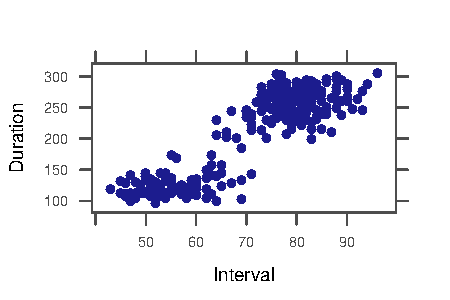
\includegraphics[width=\maxwidth]{figures/fig-unnamed-chunk-14-1} 
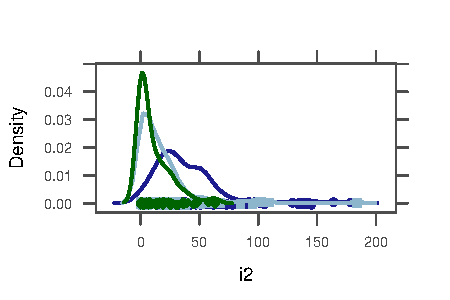
\includegraphics[width=\maxwidth]{figures/fig-unnamed-chunk-14-2} 

}



\end{knitrout}

\begin{knitrout}
\definecolor{shadecolor}{rgb}{0.969, 0.969, 0.969}\color{fgcolor}\begin{kframe}
\begin{alltt}
\hlkwd{summary}\hlstd{(drag.model)}
\end{alltt}
\begin{verbatim}
## 
## Call:
## lm(formula = log(force.drag) ~ log(velocity), data = drag)
## 
## Residuals:
##      Min       1Q   Median       3Q      Max 
## -0.34162 -0.14967 -0.04673  0.06663  0.66155 
## 
## Coefficients:
##               Estimate Std. Error t value Pr(>|t|)
## (Intercept)    2.47366    0.04425   55.91   <2e-16
## log(velocity)  2.05149    0.05366   38.23   <2e-16
## 
## Residual standard error: 0.2451 on 40 degrees of freedom
## Multiple R-squared:  0.9734,	Adjusted R-squared:  0.9727 
## F-statistic:  1462 on 1 and 40 DF,  p-value: < 2.2e-16
\end{verbatim}
\end{kframe}
\end{knitrout}
None of the p-values produced in this output is what we want.  
They are testing the hypotheses that $\beta_0=$ and that $\beta_1 = 0$.
$\beta_1 = 0$.  
But we can easily calculate the p-value we want since we have the standard error
and degrees of freedom.
\begin{knitrout}
\definecolor{shadecolor}{rgb}{0.969, 0.969, 0.969}\color{fgcolor}\begin{kframe}
\begin{alltt}
\hlstd{beta1.hat} \hlkwb{<-} \hlnum{2.051}
\hlstd{SE} \hlkwb{<-} \hlnum{0.05366}
\hlstd{t} \hlkwb{<-}  \hlstd{( beta1.hat} \hlopt{-} \hlnum{2} \hlstd{)} \hlopt{/} \hlstd{SE; t}
\end{alltt}
\begin{verbatim}
## [1] 0.9504286
\end{verbatim}
\begin{alltt}
\hlnum{2} \hlopt{*} \hlkwd{pt}\hlstd{(} \hlopt{-} \hlkwd{abs}\hlstd{(t),} \hlkwc{df}\hlstd{=} \hlnum{40} \hlstd{)}
\end{alltt}
\begin{verbatim}
## [1] 0.3476022
\end{verbatim}
\end{kframe}
\end{knitrout}
With this large a p-value, we cannot reject the null hypothesis that $p=2$.
\textbf{A large p-value does not prove that $p=2$, 
but it does say that our data are consistent with that value.}  
Of course, our data may be consistent with many other values of $p$ as well.
\end{example}

\begin{example}
	We could also do the previous example using a nonlinear model
\begin{knitrout}
\definecolor{shadecolor}{rgb}{0.969, 0.969, 0.969}\color{fgcolor}\begin{kframe}
\begin{alltt}
\hlstd{drag.model2} \hlkwb{<-} \hlkwd{nls}\hlstd{(force.drag} \hlopt{~} \hlstd{A} \hlopt{*} \hlstd{velocity}\hlopt{^}\hlstd{p,} \hlkwc{data} \hlstd{= drag,} \hlkwc{start} \hlstd{=} \hlkwd{list}\hlstd{(}\hlkwc{A} \hlstd{=} \hlnum{1}\hlstd{,} \hlkwc{p} \hlstd{=} \hlnum{2}\hlstd{))}
\hlkwd{summary}\hlstd{(drag.model2)}
\end{alltt}
\begin{verbatim}
## 
## Formula: force.drag ~ A * velocity^p
## 
## Parameters:
##   Estimate Std. Error t value Pr(>|t|)
## A 12.90528    1.61361   7.998 7.96e-10
## p  1.92989    0.09442  20.440  < 2e-16
## 
## Residual standard error: 12.48 on 40 degrees of freedom
## 
## Number of iterations to convergence: 6 
## Achieved convergence tolerance: 3.736e-06
\end{verbatim}
\end{kframe}
\end{knitrout}
Again, the p-values listed are not of interest (they are testing the hypotheses that 
each coefficient is 0).  But we can compute the p-value of interest as follows:
\begin{knitrout}
\definecolor{shadecolor}{rgb}{0.969, 0.969, 0.969}\color{fgcolor}\begin{kframe}
\begin{alltt}
\hlstd{t} \hlkwb{<-} \hlstd{(}\hlnum{2} \hlopt{-} \hlnum{1.92989}\hlstd{)}\hlopt{/}\hlnum{0.0944}
\hlstd{t}
\end{alltt}
\begin{verbatim}
## [1] 0.7426907
\end{verbatim}
\begin{alltt}
\hlnum{2} \hlopt{*} \hlkwd{pt}\hlstd{(}\hlopt{-}\hlkwd{abs}\hlstd{(t),} \hlkwc{df} \hlstd{=} \hlnum{40}\hlstd{)}
\end{alltt}
\begin{verbatim}
## [1] 0.4620085
\end{verbatim}
\end{kframe}
\end{knitrout}
Although the two p-values are different, the conclusion is the same using either model:  
Our data are consistent with the hypothesis that $p=2$.
\end{example}

\begin{example}
\begin{knitrout}
\definecolor{shadecolor}{rgb}{0.969, 0.969, 0.969}\color{fgcolor}\begin{kframe}
\begin{alltt}
\hlkwd{data}\hlstd{(PorschePrice)}
\hlkwd{head}\hlstd{(PorschePrice)}
\end{alltt}
\begin{verbatim}
##   Price Age Mileage
## 1  69.4   3    21.5
## 2  56.9   3    43.0
## 3  49.9   2    19.9
## 4  47.4   4    36.0
## 5  42.9   4    44.0
## 6  36.9   6    49.8
\end{verbatim}
\begin{alltt}
\hlstd{porsche.model} \hlkwb{<-} \hlkwd{lm}\hlstd{(Price} \hlopt{~} \hlstd{Mileage,} \hlkwc{data} \hlstd{= PorschePrice)}
\hlkwd{summary}\hlstd{(porsche.model)}
\end{alltt}
\begin{verbatim}
## 
## Call:
## lm(formula = Price ~ Mileage, data = PorschePrice)
## 
## Residuals:
##      Min       1Q   Median       3Q      Max 
## -19.3077  -4.0470  -0.3945   3.8374  12.6758 
## 
## Coefficients:
##             Estimate Std. Error t value Pr(>|t|)
## (Intercept) 71.09045    2.36986    30.0  < 2e-16
## Mileage     -0.58940    0.05665   -10.4 3.98e-11
## 
## Residual standard error: 7.17 on 28 degrees of freedom
## Multiple R-squared:  0.7945,	Adjusted R-squared:  0.7872 
## F-statistic: 108.3 on 1 and 28 DF,  p-value: 3.982e-11
\end{verbatim}
\begin{alltt}
\hlkwd{xyplot}\hlstd{(}\hlkwd{resid}\hlstd{(porsche.model)} \hlopt{~} \hlkwd{fitted}\hlstd{(porsche.model),} \hlkwc{type} \hlstd{=} \hlkwd{c}\hlstd{(}\hlstr{"p"}\hlstd{,} \hlstr{"smooth"}\hlstd{))}
\hlkwd{qqmath}\hlstd{(}\hlopt{~}\hlkwd{resid}\hlstd{(porsche.model))}
\end{alltt}
\end{kframe}

{\centering 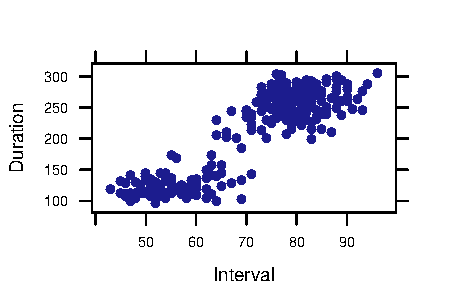
\includegraphics[width=\maxwidth]{figures/fig-unnamed-chunk-19-1} 
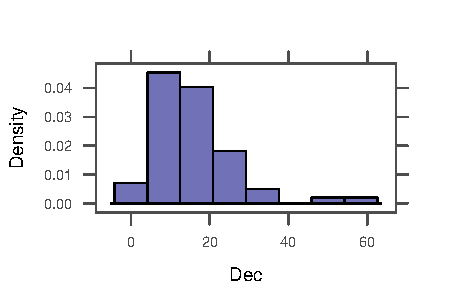
\includegraphics[width=\maxwidth]{figures/fig-unnamed-chunk-19-2} 

}



\end{knitrout}
The model looks reasonable.  What are the two hypotheses being tested?
\begin{enumerate}
	\item $H_0: \beta_0 = 0$.

		Often this is not an interesting test because often we are not so interested in
		$\beta_0$, and especially not in whether it is 0.  In this case, the intercept might
		be interesting because it tells us the price of a Porsche with no miles.  On the other hand,
		we might not expect a used car, even one with very few miles to fit the same pattern as 
		a new car.  There is probably a loss in value that occurs as soon as a car is purchased.
		
		In any case, it is clear that the intercept will not be 0; we don't need a hypothesis test
		to tell us that.  Indeed, the evidence is incredibly strong.

		A confidence interval for the intercept is more interesting since it gives a sort 
		of ``starting price'' for used Porches.
\begin{knitrout}
\definecolor{shadecolor}{rgb}{0.969, 0.969, 0.969}\color{fgcolor}\begin{kframe}
\begin{alltt}
\hlkwd{confint}\hlstd{(porsche.model)}
\end{alltt}
\begin{verbatim}
##                  2.5 %     97.5 %
## (Intercept) 66.2360186 75.9448869
## Mileage     -0.7054401 -0.4733618
\end{verbatim}
\end{kframe}
\end{knitrout}


	\item
		$H_0: \beta_1 = 0$.

		There is strong evidence against this hypothesis as well.  This is also not surprising.
		If $\beta_1 = 0$, this means that the price of the cars does not depend on the mileage.

		A test of $\beta_1=0$ in a simple linear model is often called the \term{model utility test}
		because it is testing whether the predictor is of any use to us or not.

	\item
		$H_0: \beta_1 = \beta_{10}$.

		Although the output above doesn't do all of the work for us, we can test other
		hypotheses as well.  (The notation above is a bit tricky, $\beta_{10}$ should be read
		``$\beta_1$ null" -- it is a hypothesized value for $\beta_1$.)
		
		For example, let's test $\beta_1 = -1$.  That the hypothesis that the value 
		drops one dollar per mile driven.

\begin{knitrout}
\definecolor{shadecolor}{rgb}{0.969, 0.969, 0.969}\color{fgcolor}\begin{kframe}
\begin{alltt}
\hlstd{t} \hlkwb{<-} \hlstd{(}\hlopt{-}\hlnum{0.5894} \hlopt{-} \hlstd{(}\hlopt{-}\hlnum{1}\hlstd{) )} \hlopt{/} \hlnum{0.566}\hlstd{; t}
\end{alltt}
\begin{verbatim}
## [1] 0.7254417
\end{verbatim}
\begin{alltt}
\hlnum{2} \hlopt{*} \hlkwd{pt}\hlstd{(} \hlopt{-} \hlkwd{abs}\hlstd{(t),} \hlkwc{df}\hlstd{=}\hlnum{28} \hlstd{)}
\end{alltt}
\begin{verbatim}
## [1] 0.4742011
\end{verbatim}
\end{kframe}
\end{knitrout}
The small p-value would lead us to reject this value for $\beta_1$.
\end{enumerate}
\end{example}

\section{Connection to Confidence Intervals}
\label{sec:CI-HT-duality}

There is a natural duality between t-based hypothesis tests and confidence intervals.
Since the p-value is computed using tail probabilities of the t-distribution and confidence
level describes the central probability, the p-value will be below 0.05 exactly when the 
hypothesized value is not contained in the 95\% confidence interval.  (Similar statements can
be made for other confidence levels.)
%So a confidence interval generally conveys more information than a p-value in these situations.

\begin{example}
	In the preceding example we rejected the null hypothesis that $\beta_1 = -1$.
In fact, we will reject (at the $alpha=0.05$ level) any hypothesized value not contained 
in the 95\% confidence interval.
\begin{knitrout}
\definecolor{shadecolor}{rgb}{0.969, 0.969, 0.969}\color{fgcolor}\begin{kframe}
\begin{alltt}
\hlstd{t} \hlkwb{<-} \hlstd{(}\hlopt{-}\hlnum{0.5894} \hlopt{-} \hlstd{(}\hlopt{-}\hlnum{0.75}\hlstd{))}\hlopt{/}\hlnum{0.566}
\hlstd{t}
\end{alltt}
\begin{verbatim}
## [1] 0.2837456
\end{verbatim}
\begin{alltt}
\hlnum{2} \hlopt{*} \hlkwd{pt}\hlstd{(}\hlopt{-}\hlkwd{abs}\hlstd{(t),} \hlkwc{df} \hlstd{=} \hlnum{28}\hlstd{)}
\end{alltt}
\begin{verbatim}
## [1] 0.778693
\end{verbatim}
\end{kframe}
\end{knitrout}
But we won't reject values inside the confidence interval.
\begin{knitrout}
\definecolor{shadecolor}{rgb}{0.969, 0.969, 0.969}\color{fgcolor}\begin{kframe}
\begin{alltt}
\hlstd{t} \hlkwb{<-} \hlstd{(}\hlopt{-}\hlnum{0.5894} \hlopt{-} \hlstd{(}\hlopt{-}\hlnum{0.7}\hlstd{))}\hlopt{/}\hlnum{0.566}
\hlstd{t}
\end{alltt}
\begin{verbatim}
## [1] 0.1954064
\end{verbatim}
\begin{alltt}
\hlnum{2} \hlopt{*} \hlkwd{pt}\hlstd{(}\hlopt{-}\hlkwd{abs}\hlstd{(t),} \hlkwc{df} \hlstd{=} \hlnum{28}\hlstd{)}
\end{alltt}
\begin{verbatim}
## [1] 0.846486
\end{verbatim}
\end{kframe}
\end{knitrout}
\end{example}


\begin{example}
	The output below illustrates this duality.
\begin{knitrout}
\definecolor{shadecolor}{rgb}{0.969, 0.969, 0.969}\color{fgcolor}\begin{kframe}
\begin{alltt}
\hlstd{drag.model}
\end{alltt}
\begin{verbatim}
## 
## Call:
## lm(formula = log(force.drag) ~ log(velocity), data = drag)
## 
## Coefficients:
##   (Intercept)  log(velocity)  
##         2.474          2.051
\end{verbatim}
\begin{alltt}
\hlkwd{confint}\hlstd{(drag.model)}
\end{alltt}
\begin{verbatim}
##                  2.5 %   97.5 %
## (Intercept)   2.384238 2.563088
## log(velocity) 1.943045 2.159941
\end{verbatim}
\end{kframe}
\end{knitrout}
Since the confidence interval for $p$ (i.e., for $\beta_1$) includes 2, 
2 is a plausible value for the power (i.e., consistent with our data).
A p-value larger than 0.05 says the same thing at the same level of confidence.  
\end{example}

\begin{problem}
	An experiment was conducted to see if the number of clicks 
	on a Geiger counter in a 7.5 minute interval is related to
	the distance (in m) between a radioactive source and the detection 
	device according to an inverse square law:
	\[
	\mbox{clicks} =	A + \frac{k}{\mbox{distance}^{2}}
	\]
	Answer the questions below using the following output

\begin{knitrout}
\definecolor{shadecolor}{rgb}{0.969, 0.969, 0.969}\color{fgcolor}\begin{kframe}
\begin{alltt}
\hlstd{model} \hlkwb{<-} \hlkwd{lm}\hlstd{(clicks} \hlopt{~} \hlkwd{I}\hlstd{(}\hlnum{1}\hlopt{/}\hlstd{(distance}\hlopt{^}\hlnum{2}\hlstd{)),} \hlkwc{data} \hlstd{= Geiger)}
\hlkwd{summary}\hlstd{(model)}
\end{alltt}
\begin{verbatim}
## 
## Call:
## lm(formula = clicks ~ I(1/(distance^2)), data = Geiger)
## 
## Residuals:
##     Min      1Q  Median      3Q     Max 
## -32.234 -15.817   4.027  10.899  34.091 
## 
## Coefficients:
##                   Estimate Std. Error t value Pr(>|t|)
## (Intercept)        114.281     10.787   10.59 5.51e-06
## I(1/(distance^2))   31.477      1.001   31.46 1.13e-09
## 
## Residual standard error: 22.51 on 8 degrees of freedom
## Multiple R-squared:  0.992,	Adjusted R-squared:  0.991 
## F-statistic: 989.7 on 1 and 8 DF,  p-value: 1.134e-09
\end{verbatim}
\begin{alltt}
\hlkwd{plot}\hlstd{(model,} \hlkwc{w} \hlstd{=} \hlnum{1}\hlopt{:}\hlnum{2}\hlstd{)}
\end{alltt}
\end{kframe}

{\centering 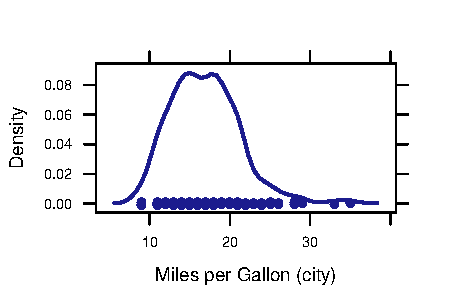
\includegraphics[width=\maxwidth]{figures/fig-unnamed-chunk-26-1} 
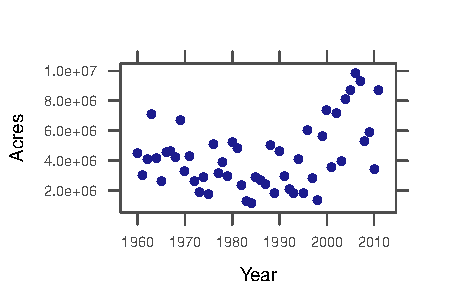
\includegraphics[width=\maxwidth]{figures/fig-unnamed-chunk-26-2} 

}



\end{knitrout}
\begin{enumerate}
	\item
		Are there are any reasons (from what you can tell in the output
		above) to be concerned about using this model?
	\item
		What does $A$ tell us about this situation?  
		What would it mean if $A$ were 0?  What if $A \neq 0$?
\item
	What is the estimate for $A$?  Express this as an estimate $\pm$ uncertainty
	using our rules for numbers of digits.
\item
	What is the p-value for the test of the null hypothesis that $A=0$?
	What conclusion do we draw from this?
\item
	What does $k$ tell us about this situation?  In what situations would $k$
	be larger or smaller?  What would it mean if $k$ were 0?

	\item
		Express the estimate for $k$ as an estimate $\pm$ uncertainty.
\item
	What is the p-value for the test of the null hypothesis that $k=0$?
	What conclusion do we draw from this?
\item
A standard radioactive substance has a value of $k=29.812$.  Might that be the
substance we are using here?  Conduct an appropriate hypothesis test to answer
this question.  Carefully show all four steps.
\end{enumerate}
\end{problem}

\begin{solution}
	\begin{enumerate}
			\item
				The normal-quantile plot looks pretty good for a sample of this size.
				The residual plot is not as ``noisy'' as we would like (the first few residuals
				cluster above zero, then next few below.  Ideally we would like to have a larger 
				data set to see whether this pattern persists or whether things "fill-in" with more
				data.
			\item
				$A$ is a measure of background radiation levels, it is the amount of clicks 
				we would get if our test substance were ``at infinity'', i.e., so far away (or 
				beyond some shielding) that it does not affect the Geiger counter.
			\item
				$114 \pm 11$
			\item
				\ensuremath{5.5\times 10^{-6}}.  This gives strong evidence that there some background radiation
				being measured by the Geiger counter.
			\item
				$k$ measures the rate at which our test substance is emitting radioactive 
				particles.  If $k$ is 0, then our substance is not radioactive (or at least not
				being detected by the Geiger counter).
			\item
				$31.5  \pm 1.0$
			\item
				\ensuremath{1.1\times 10^{-9}}.  We have strong evidence that our substance is decaying and 
				contributing to the Geiger counter clicks.
			\item
				$H_0: k = 29.812$;  $H_a: k \neq 29.812$
\begin{knitrout}
\definecolor{shadecolor}{rgb}{0.969, 0.969, 0.969}\color{fgcolor}\begin{kframe}
\begin{alltt}
\hlstd{t} \hlkwb{<-} \hlstd{(}\hlnum{31.5} \hlopt{-} \hlnum{29.812}\hlstd{)}\hlopt{/}\hlnum{1}
\hlstd{t}  \hlcom{# test statistic}
\end{alltt}
\begin{verbatim}
## [1] 1.688
\end{verbatim}
\begin{alltt}
\hlnum{2} \hlopt{*} \hlkwd{pt}\hlstd{(}\hlopt{-}\hlkwd{abs}\hlstd{(t),} \hlkwc{df} \hlstd{=} \hlnum{8}\hlstd{)}  \hlcom{# p -value}
\end{alltt}
\begin{verbatim}
## [1] 0.1298892
\end{verbatim}
\end{kframe}
\end{knitrout}
				Conclusion.  With a p-value this large, we cannot reject the null hypothesis.
				Our data are consistent with the hypothesis that our test substance is the same
				as the standard substance.
	\end{enumerate}
\end{solution}


\begin{problem} %[title=Gentleman Tasting Wine]
\myindex{wine!gentleman tasting|probidx}%
  A gentleman claims he can distinguish between four vintages of 
  a particular wine.  His friends, assuming he has probably just 
  had too much of each, decide to test him.  They prepare one glass
  of each vintage and present the gentleman with four unlabeled glasses
  of wine.  What is the probability that the gentleman correctly 
  identifies all four simply by guessing?
\end{problem}

\begin{solution}
  The wines can be presented in $4 \cdot 3 \cdot 2 \cdot 1 = 24$ different
  orders, so the probability of guessing correctly is $1/24$.
\end{solution}

\begin{problem}
\label{prob:drag-refit}
	Redo the drag force analysis after removing observations that appear not to have reached
	terminal velocity.

	If you can describe the rows you want to remove logically, the \function{subset()} command
	works well for this.  You can also remove rows by row number.  For example, the following
	removes rows 1, 3, 5 and 7:
\begin{knitrout}
\definecolor{shadecolor}{rgb}{0.969, 0.969, 0.969}\color{fgcolor}\begin{kframe}
\begin{alltt}
\hlstd{drag[}\hlopt{-}\hlkwd{c}\hlstd{(}\hlnum{1}\hlstd{,} \hlnum{3}\hlstd{,} \hlnum{5}\hlstd{,} \hlnum{7}\hlstd{), ]}
\end{alltt}
\end{kframe}
\end{knitrout}
\end{problem}

\begin{solution}
Let's remove the fastest values at each setting.  Although they are the fastest, it appears 
that terminal velocity has not yet been reached.  At least, these points would fit the 
overall pattern better if the velocity were larger.
\begin{knitrout}
\definecolor{shadecolor}{rgb}{0.969, 0.969, 0.969}\color{fgcolor}\begin{kframe}
\begin{alltt}
\hlkwd{xyplot}\hlstd{(force.drag} \hlopt{~} \hlstd{velocity,} \hlkwc{data} \hlstd{= drag,} \hlkwc{groups} \hlstd{= (velocity} \hlopt{<} \hlnum{3.9}\hlstd{)} \hlopt{& !}\hlstd{(velocity} \hlopt{>} \hlnum{1} \hlopt{&} \hlstd{velocity} \hlopt{<}
    \hlnum{1.5}\hlstd{))}
\hlstd{drag2} \hlkwb{<-} \hlkwd{subset}\hlstd{(drag, (velocity} \hlopt{<} \hlnum{3.9}\hlstd{)} \hlopt{& !}\hlstd{(velocity} \hlopt{>} \hlnum{1} \hlopt{&} \hlstd{velocity} \hlopt{<} \hlnum{1.5}\hlstd{))}
\end{alltt}
\end{kframe}

{\centering 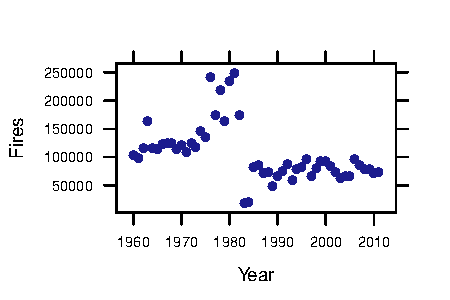
\includegraphics[width=\maxwidth]{figures/fig-unnamed-chunk-29-1} 

}



\end{knitrout}
\begin{knitrout}
\definecolor{shadecolor}{rgb}{0.969, 0.969, 0.969}\color{fgcolor}\begin{kframe}
\begin{alltt}
\hlstd{drag2.model} \hlkwb{<-} \hlkwd{lm}\hlstd{(}\hlkwd{log}\hlstd{(force.drag)} \hlopt{~} \hlkwd{log}\hlstd{(velocity),} \hlkwc{data} \hlstd{= drag2)}
\hlkwd{summary}\hlstd{(drag2.model)}
\end{alltt}
\begin{verbatim}
## 
## Call:
## lm(formula = log(force.drag) ~ log(velocity), data = drag2)
## 
## Residuals:
##      Min       1Q   Median       3Q      Max 
## -0.31581 -0.10503  0.01792  0.08009  0.25424 
## 
## Coefficients:
##               Estimate Std. Error t value Pr(>|t|)
## (Intercept)    2.36586    0.02722   86.93   <2e-16
## log(velocity)  2.11416    0.03679   57.46   <2e-16
## 
## Residual standard error: 0.1367 on 28 degrees of freedom
## Multiple R-squared:  0.9916,	Adjusted R-squared:  0.9913 
## F-statistic:  3302 on 1 and 28 DF,  p-value: < 2.2e-16
\end{verbatim}
\begin{alltt}
\hlkwd{plot}\hlstd{(drag2.model,} \hlkwc{w} \hlstd{=} \hlnum{1}\hlopt{:}\hlnum{2}\hlstd{)}
\end{alltt}
\end{kframe}

{\centering 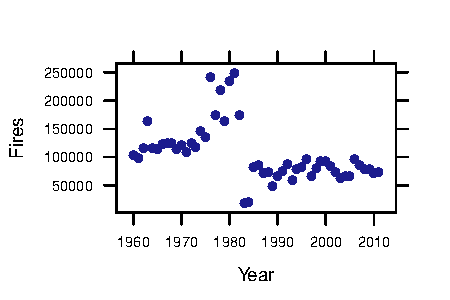
\includegraphics[width=\maxwidth]{figures/fig-unnamed-chunk-30-1} 
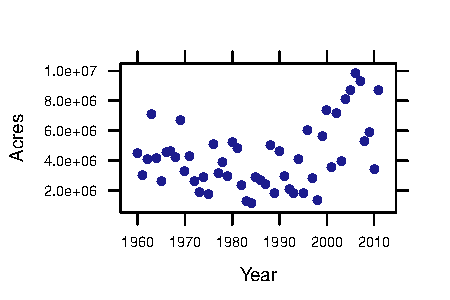
\includegraphics[width=\maxwidth]{figures/fig-unnamed-chunk-30-2} 

}



\end{knitrout}
The model is still not as good as we might like, and it seams like the fit is different for the 
heavier objects than for the lighter ones.  This could be due to some flaw in the design of the 
experiment or because drag force actually behaves differently at low speeds vs. higher speeds.
Notice the data suggest an exponent on velocity that is just a tiny bit larger than 2:
\begin{knitrout}
\definecolor{shadecolor}{rgb}{0.969, 0.969, 0.969}\color{fgcolor}\begin{kframe}
\begin{alltt}
\hlkwd{confint}\hlstd{(drag2.model)}
\end{alltt}
\begin{verbatim}
##                  2.5 %   97.5 %
## (Intercept)   2.310110 2.421611
## log(velocity) 2.038795 2.189534
\end{verbatim}
\end{kframe}
\end{knitrout}
So our data (for whichever reason, potentially still due to design issues) is not compatible 
with the hypothesis that this exponent should be 2.
\end{solution}

\begin{problem}
	Sixteen samples of a certain brand of hydrogenated vegetable oil were tested to determine 
	their melting point.  The mean melting point for the 16 samples was 94.32 degrees 
	and the standard deviation was 1.2 degrees.

	\begin{enumerate}
		\item
    Conduct a test of the hypothesis $\mu = 95$.  Follow the four step procedure.
\item
	Will 95 be inside or outside of a 95\% confidence interval for the melting point?
	How do you know?
	\end{enumerate}
\end{problem}

\begin{solution}
\begin{knitrout}
\definecolor{shadecolor}{rgb}{0.969, 0.969, 0.969}\color{fgcolor}\begin{kframe}
\begin{alltt}
\hlstd{SE} \hlkwb{<-} \hlnum{1.2} \hlopt{/} \hlkwd{sqrt}\hlstd{(}\hlnum{16}\hlstd{); SE}
\end{alltt}
\begin{verbatim}
## [1] 0.3
\end{verbatim}
\begin{alltt}
\hlstd{t} \hlkwb{<-} \hlstd{(}\hlnum{94.32} \hlopt{-} \hlnum{95}\hlstd{)} \hlopt{/} \hlstd{SE; t}
\end{alltt}
\begin{verbatim}
## [1] -2.266667
\end{verbatim}
\begin{alltt}
\hlstd{p_val} \hlkwb{<-} \hlnum{2} \hlopt{*} \hlkwd{pt}\hlstd{(} \hlopt{-} \hlkwd{abs}\hlstd{(t),} \hlkwc{df}\hlstd{=}\hlnum{15} \hlstd{); p_val}    \hlcom{# p-value}
\end{alltt}
\begin{verbatim}
## [1] 0.03862989
\end{verbatim}
\end{kframe}
\end{knitrout}
	95 will be 
	outside 
	the confidence interval because the p-value is 
	less than 0.05. 
	As a double check, here is the 95\% confidence interval.
\begin{knitrout}
\definecolor{shadecolor}{rgb}{0.969, 0.969, 0.969}\color{fgcolor}\begin{kframe}
\begin{alltt}
\hlstd{t_star} \hlkwb{<-} \hlkwd{qt}\hlstd{(}\hlnum{0.975}\hlstd{,} \hlkwc{df} \hlstd{=} \hlnum{11}\hlstd{)}
\hlstd{t_star}
\end{alltt}
\begin{verbatim}
## [1] 2.200985
\end{verbatim}
\begin{alltt}
\hlnum{94.32} \hlopt{+} \hlkwd{c}\hlstd{(}\hlopt{-}\hlnum{1}\hlstd{,} \hlnum{1}\hlstd{)} \hlopt{*} \hlstd{t_star} \hlopt{*} \hlstd{SE}
\end{alltt}
\begin{verbatim}
## [1] 93.6597 94.9803
\end{verbatim}
\end{kframe}
\end{knitrout}
\end{solution}

\begin{problem}
	The Charpy V-notch impact test is the basis for sutdy many amterial toughness criteria.
	This test was applied to 42 specimens of a particular alloy at 110 degrees F.
	The mean amount of transverse lateral expansion was computed to be
	73.1 mils with a sample standard deviation of 5.9 mils.

	To be suitable for a particular application, the true amount of expansion must be less than 75 mils.
	The alloy will not be used unless their is strong evidence (a p-value below 0.01) that 
	this specification is met.

	\begin{enumerate}
		\item
			Use a p-value to decide whether this alloy may be used.
		\item
			Use a confidence interval to decide whether this alloy may be used.
		\item
			Are there advantages to one approach over the other?  If you had to present
			an argument to your boss, which approach would you use?
	\end{enumerate}
\end{problem}

\begin{solution}
	\begin{enumerate}
		\item
			In this situation it makes sense to do a one-sided test since we will reject
			the alloy only if the amount of expansion is to high, not if it is too low.
\begin{knitrout}
\definecolor{shadecolor}{rgb}{0.969, 0.969, 0.969}\color{fgcolor}\begin{kframe}
\begin{alltt}
\hlstd{SE} \hlkwb{<-} \hlnum{5.9}\hlopt{/}\hlkwd{sqrt}\hlstd{(}\hlnum{42}\hlstd{); SE}
\end{alltt}
\begin{verbatim}
## [1] 0.9103898
\end{verbatim}
\begin{alltt}
\hlstd{t} \hlkwb{<-} \hlstd{(}\hlnum{73.1} \hlopt{-} \hlnum{75}\hlstd{)} \hlopt{/} \hlstd{SE; t}
\end{alltt}
\begin{verbatim}
## [1] -2.087018
\end{verbatim}
\begin{alltt}
\hlkwd{pt}\hlstd{(t,} \hlkwc{df}\hlstd{=}\hlnum{41}\hlstd{)}
\end{alltt}
\begin{verbatim}
## [1] 0.02157239
\end{verbatim}
\end{kframe}
\end{knitrout}
		\item
			Corresponding to a 1-sided test with a significance level of $\alpha = 0.01$,
			we could make a 98\% confidence interval (1\% in each tail).  The upper end of this
			would be the same as for a 1-sided 99\% confidence interval
\begin{knitrout}
\definecolor{shadecolor}{rgb}{0.969, 0.969, 0.969}\color{fgcolor}\begin{kframe}
\begin{alltt}
\hlstd{t_star} \hlkwb{<-} \hlkwd{qt}\hlstd{(}\hlnum{0.99}\hlstd{,} \hlkwc{df} \hlstd{=} \hlnum{41}\hlstd{)}
\hlnum{73.1} \hlopt{+} \hlkwd{c}\hlstd{(}\hlopt{-}\hlnum{1}\hlstd{,} \hlnum{1}\hlstd{)} \hlopt{*} \hlstd{t_star} \hlopt{*} \hlstd{SE}
\end{alltt}
\begin{verbatim}
## [1] 70.89613 75.30387
\end{verbatim}
\end{kframe}
\end{knitrout}
		\item
			If all we are interested in is a decision, the two methods are equivalent.
			I confidence interval might be easier to explain to someone less familiar with
			statistics.
	\end{enumerate}

\end{solution}

\begin{problem}
	Data from a 1993 study to see how well lichens serve as an indicator for air pollution are in the 
	\dataframe{ex12.20} data set in the \pkg{Devore6} package. 
	In that paper, a simple linear model was fit to see how the wet deposition of $NO^{-}_3$ 
	related to the percentage dry weight of lichen.
	Using this model, 
	\begin{enumerate}
		\item
			Test the hypothesis that the slope of the linear relationship is 1.
		\item
			Compute a 90\% confidence interval for the slope of the linear relationship.
	\end{enumerate}
\begin{knitrout}
\definecolor{shadecolor}{rgb}{0.969, 0.969, 0.969}\color{fgcolor}\begin{kframe}
\begin{alltt}
\hlkwd{require}\hlstd{(Devore6)}
\hlkwd{summary}\hlstd{(}\hlkwd{lm}\hlstd{(LichenN} \hlopt{~} \hlstd{deposition,} \hlkwc{data} \hlstd{= ex12.20))}
\end{alltt}
\begin{verbatim}
## 
## Call:
## lm(formula = LichenN ~ deposition, data = ex12.20)
## 
## Residuals:
##      Min       1Q   Median       3Q      Max 
## -0.20283 -0.14691 -0.02255  0.06655  0.44541 
## 
## Coefficients:
##             Estimate Std. Error t value Pr(>|t|)
## (Intercept)  0.36510    0.09904   3.686 0.003586
## deposition   0.96683    0.18292   5.286 0.000258
## 
## Residual standard error: 0.1932 on 11 degrees of freedom
## Multiple R-squared:  0.7175,	Adjusted R-squared:  0.6918 
## F-statistic: 27.94 on 1 and 11 DF,  p-value: 0.0002581
\end{verbatim}
\end{kframe}
\end{knitrout}
\end{problem}
\begin{solution}
\begin{knitrout}
\definecolor{shadecolor}{rgb}{0.969, 0.969, 0.969}\color{fgcolor}\begin{kframe}
\begin{alltt}
\hlstd{t} \hlkwb{<-} \hlstd{(}\hlnum{0.967} \hlopt{-} \hlnum{1}\hlstd{)} \hlopt{/} \hlnum{0.183}
\hlnum{2} \hlopt{*} \hlkwd{pt}\hlstd{(} \hlopt{-}\hlkwd{abs}\hlstd{(t),} \hlkwc{df}\hlstd{=}\hlnum{11} \hlstd{)}           \hlcom{# p-value}
\end{alltt}
\begin{verbatim}
## [1] 0.8601744
\end{verbatim}
\end{kframe}
\end{knitrout}
With such a large p-value, we do not reject the null hypothesis.  Our data are consistent 
with the hypothesis that the slope is 1.
\begin{knitrout}
\definecolor{shadecolor}{rgb}{0.969, 0.969, 0.969}\color{fgcolor}\begin{kframe}
\begin{alltt}
\hlstd{t_star} \hlkwb{<-} \hlkwd{qt}\hlstd{(}\hlnum{0.95}\hlstd{,} \hlkwc{df} \hlstd{=} \hlnum{11}\hlstd{)}
\hlstd{t_star}
\end{alltt}
\begin{verbatim}
## [1] 1.795885
\end{verbatim}
\begin{alltt}
\hlnum{0.967} \hlopt{+} \hlkwd{c}\hlstd{(}\hlopt{-}\hlnum{1}\hlstd{,} \hlnum{1}\hlstd{)} \hlopt{*} \hlstd{t_star} \hlopt{*} \hlnum{0.183}  \hlcom{# 90% CI}
\end{alltt}
\begin{verbatim}
## [1] 0.6383531 1.2956469
\end{verbatim}
\end{kframe}
\end{knitrout}
Notice that this interval includes 1.  We knew it would because 1 would not be rejected at the 
$\alpha = 0.10$ level.
\begin{knitrout}
\definecolor{shadecolor}{rgb}{0.969, 0.969, 0.969}\color{fgcolor}\begin{kframe}
\begin{alltt}
\hlstd{t_star} \hlkwb{<-} \hlkwd{qt}\hlstd{(}\hlnum{0.975}\hlstd{,} \hlkwc{df} \hlstd{=} \hlnum{11}\hlstd{)}
\hlnum{95} \hlopt{+} \hlkwd{c}\hlstd{(}\hlopt{-}\hlnum{1}\hlstd{,} \hlnum{1}\hlstd{)} \hlopt{*} \hlstd{t_star} \hlopt{*} \hlstd{SE}
\end{alltt}
\begin{verbatim}
## [1] 92.99625 97.00375
\end{verbatim}
\end{kframe}
\end{knitrout}
\end{solution}

\newpage
\section*{Exercises}
\shipoutProblems


\ifsolutions
%\ifsolutionslocal
\newpage
\section*{Solutions}
\shipoutSolutions
%\fi
\fi
\bibliographystyle{amsalpha}
\bibliography{StatsBook,DataSets,jamstatassoc,RS,R,kaplan}
\end{document}
